\chapter[Experimental Setup and Evaluation]{Experimental Setup \newline and Evaluation}

\section{Dataset Construction} \label{datasetConstruction}

In order to test the effectiveness of the machine learning algorithms and natural language processing techniques discussed in Chapter 2, we constructed a corpus of malicious and credible articles.  The malicious articles used in our dataset were all stories that had trended on social media that Snopes eventually investigated and labelled false.  A list of URLs to these articles was later compiled by Allcott and Gentzkow for their study on the impact of fake news on the 2016 presidential election \cite{gentzkow}.  After Dr. Gentzkow and his research assistant, Chuan Yu, provided us with this list, we designed a script to scrape the content of the article on each web page.  Of the 948 fake news URLs, just 478 articles that had gone live between January and December 2016 were still available at the start of this study (March 2017).

To compile a list of URLs to credible articles, we used the Google News search engine to query for news articles published by major news organizations.  In order to ensure that all the credible articles would be similar to the set of articles available during the campaign season, a few filters were applied to each query.  First, the keywords "trump", "clinton", and "election" were conjoined together with OR operators in each query to only capture articles related to the 2016 presidential election.  Next, a date range restriction from January 1, 2016 to December 1, 2016 was imposed on the query in ensure that the timespan of the credible corpus would be similar to that of the malicious corpus.  Finally, a Google News source filter was applied to the query to restrict the result set to articles that had actually been published by each of the following major news outlets: ABC, BBC, CBS, CNN, FOX, NY Times, Reuters, and Washington Post.

As shown in Fig. \ref{fig:googlenews}, the search results from Google News is not a list of URLs, but rather enriched content that includes thumbnails, articles' titles as hyperlinks, and short blurbs from each article.  Thus, a results page crawler was created to traverse through and extract the direct URLs from the first 17 pages of results returned by the aforementioned query for each news organization.  Once the crawler had curated a list of URLs to credible news articles, each corresponding web page was scraped for its news content.  At the end of this stage, 1226 credible articles had been successfully downloaded.


\begin{figure}[h]
\centering
\captionsetup{justification=centering,width=0.95\textwidth}
\centerline{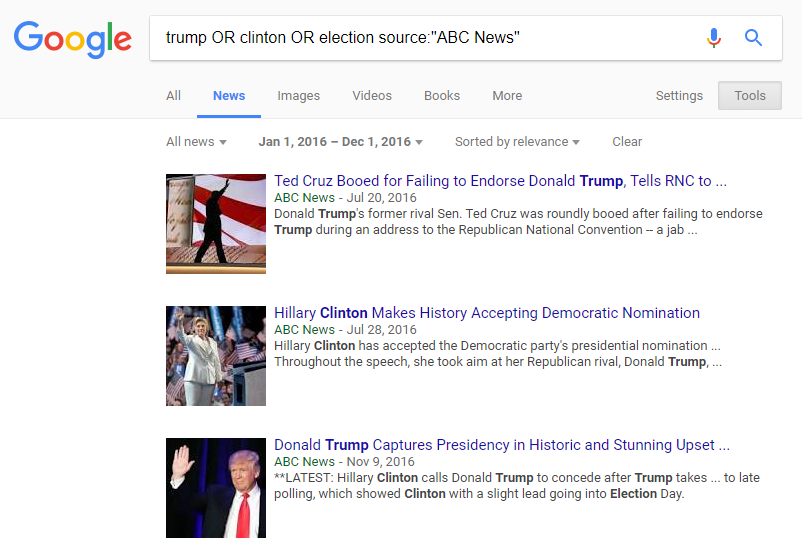
\includegraphics[width=0.95\textwidth]{googlenews.png}}
\caption[ABC News Articles On Google News]{
    Google News query results for articles published by ABC News between January 1, 2016 and December 1, 2016
}
\label{fig:googlenews}
\end{figure}


Hoping to reap the benefits of sentiment analysis that were discussed in Section \ref{sentimentAnalysisSection}, sentiment-related features for each document were added to the dataset using Google Cloud's Natural Language API and Microsoft Azure's Text Analytics API.  Though both APIs provide a sentiment score for each input document, their scores span across different ranges: Google's score lies between -1 and 1, and Microsoft's score lies between 0 and 1.  However, both APIs do indicate negative texts with low scores, and positive texts with high scores \cite{googleSentiment,microsoftSentiment}.  From here on out, an article is deemed negative if its Google sentiment score is less than -0.25 or if its Microsoft sentiment score is less than 0.375.  An article is considered positive if its Google sentiment score is greater than 0.25, or if its Microsoft sentiment score is greater than 0.625.  Additionally, we define polar articles as articles that are either negative or positive according to either API's sentiment score.

The other feature that the Google Cloud Natural Language API provides is the overall sentiment magnitude for the input text.  This magnitude, which ranges from 0 to infinity, indicates the overall strength of emotion in the text.  That is, each emotional word, whether it's positive or negative, additively contributes to the magnitude.  One drawback to this feature is that it is not normalized; thus, a document with a mix of sentiment and sentiment score close to 0 could potentially have a sentiment magnitude that is greater than the sentiment magnitude of a polar article simply because the mixed document is larger \cite{googleSentiment}.

To refine the overall dataset, duplicate documents and documents very similar to another document with the same label were eliminated.  To determine which documents are similar to others, a cosine similarity matrix of similarity scores (using tf-idf vector representation) between each pair of documents was constructed.  For each pair of documents with a similarity score greater than 0.90, the document that consisted of the least words was excluded from the dataset under the assumption that it was an article that simply quoting large chunks of the other with very little analysis.

After pruning the duplicate articles, a total of 333 malicious and 1008 credible articles remained.  In order create valid training and testing sets that reflected a possible real-world scenario, the dataset was ordered and split by date of publication.  That is, every article that was published before October 13, 2016 was moved into the training set, and every article that was published from October 13, 2016 and onwards was placed in the testing set.  Therefore, the training set is composed of the 774 of the earliest credible articles and 207 of the earliest malicious articles, and the testing set is composed of 234 of the newest credible articles and 126 of the newest malicious articles.  However, to further combat overfitting, a tuning set was ultimately broken off from the later 20\% of the training set; i.e., 154 of the latest credible articles and 41 of the latest malicious articles were removed from the training set and placed into the tuning set (a.k.a. validation set).  Thus, the actual training set consists of 620 oldest credible articles, and the 166 oldest malicious articles.


\section{Data Exploration} \label{dataExploration}

To determine which features may be the most effective for classification, the following plots are constructed to visualize the relationship between select features of the malicious and credible articles.


\begin{figure}[h!]
\centering
\captionsetup{justification=centering,width=0.95\textwidth}
\centerline{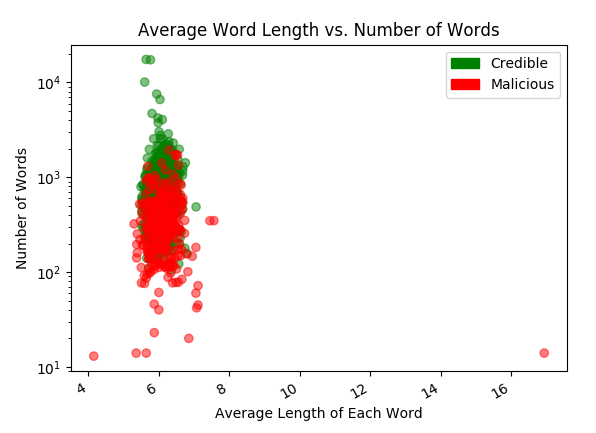
\includegraphics[scale=0.65]{wordlenNumWordsLogScale.png}}
\caption[Average Word Length vs Number of Words]{
    A plot of the average word length of each document and number of words in each document
}
\label{fig:wordlenNumWordsLogScale}
\end{figure}


\begin{figure}[h!]
\centering
\captionsetup{justification=centering,width=0.95\textwidth}
\centerline{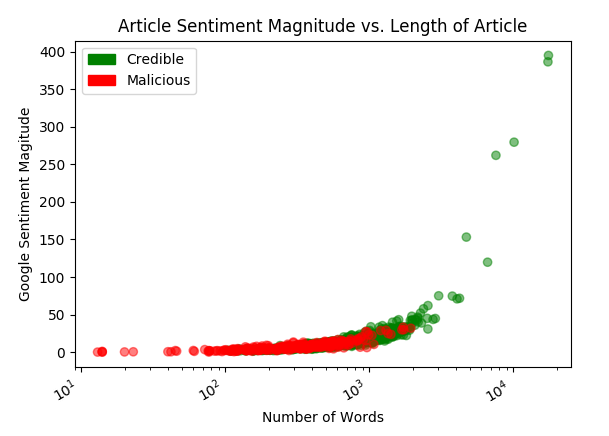
\includegraphics[scale=0.65]{sentimentMagnitude_vs_ArticleLen.png}}
\caption[Number of Words vs Google Sentiment Magnitude]{
    A plot of the number of words in each document and the Google sentiment magnitude of each document
}
\label{fig:numWordsToSentimentMagnitude}
\end{figure}


Fig. \ref{fig:wordlenNumWordsLogScale} shows the relationship between the average length of each word (i.e., the number of characters) in an article, and the number of words in the article.  Note that Fig. \ref{fig:wordlenNumWordsLogScale} has an outlier, all the way to right, representing a document with very long words, but with a few number of words.  This document that has an average word length greater than 16 characters exemplifies the wide range of styles for maliciously written web pages that pose as articles.  In fact, this particular document exhibits very few words, and simply points the reader to other links and tweets.

Fig. \ref{fig:numWordsToSentimentMagnitude} exemplifies the effect that the length of the document has on the Google sentiment magnitude.  As hypothesized before, larger documents tend to have a greater sentiment magnitude.  In fact, almost all of the credible articles that are longer than the longest malicious article has a sentiment magnitude greater than the sentiment magnitude of every malicious article.


\begin{figure}
\centering
\captionsetup{justification=centering,width=0.95\textwidth}
    \begin{subfigure}[h]{0.5\textwidth}
            \centering
            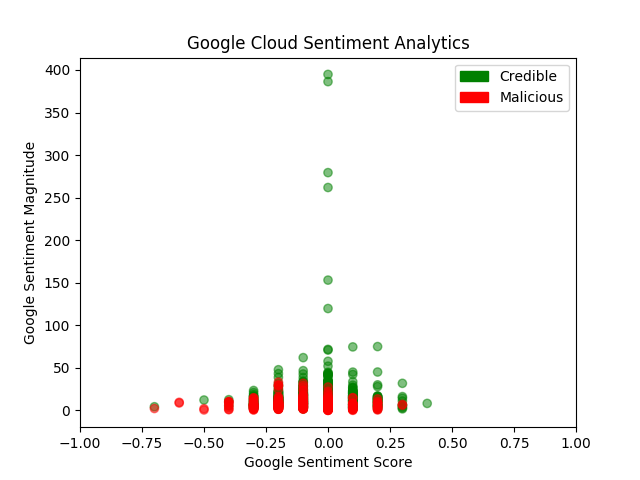
\includegraphics[width=\linewidth]{googleCloudSentiment.png}
            \caption[Google Sentiment Score vs Magnitude]{
                 Google Cloud Natural Language API 
            }
            \label{fig:googleCloudSentiment}
    \end{subfigure}\hfill
    \begin{subfigure}[h]{0.5\textwidth}
            \centering
            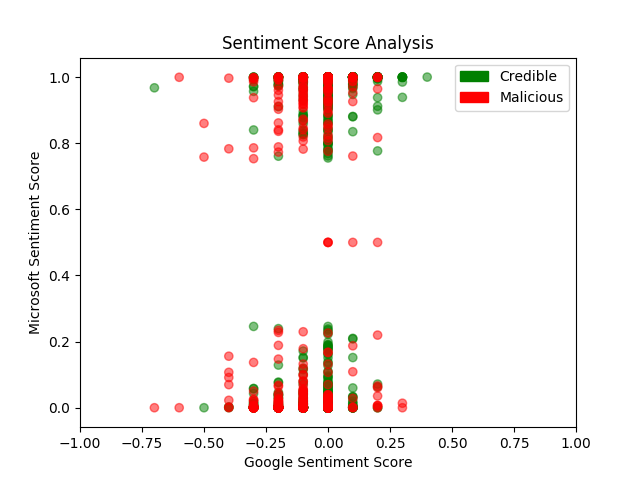
\includegraphics[width=\linewidth]{sentimentScoreAnalysis.png}
            \caption[Sentiment Scores: Google vs Microsoft]{
                Both APIs' sentiment scores
            }
            \label{fig:googleMicrosoftSentiment}
    \end{subfigure}\hfill
    \caption[Sentiment Analysis API Results]{
        Sentiment analysis results using Google Cloud and Microsoft Azure APIs
    }
\label{fig:sentimentScoreAnalysis}
\end{figure}


Fig. \ref{fig:googleCloudSentiment} depicts the shared relationship between the articles' Google sentiment score and magnitude, and Fig. \ref{fig:googleMicrosoftSentiment} shows the discrepancies between the sentiment scores according to different Google and Microsoft APIs.  If both sentiment analysis APIs were in complete agreement, the scatter plot would be roughly linear; i.e., articles attributed with a low Google sentiment score (approximately -1) should also have a correspondingly low correspond Microsoft sentiment score (approximately 0).  Even though the values seem contradictory at times, these features are kept in the dataset and the classifiers are charged with the task of learning appropriate weights for each feature in order to produce accurate predictions.


\begin{figure}
\centering
\captionsetup{justification=centering,width=0.95\textwidth}
    \begin{subfigure}[h]{0.5\textwidth}
            \centering
            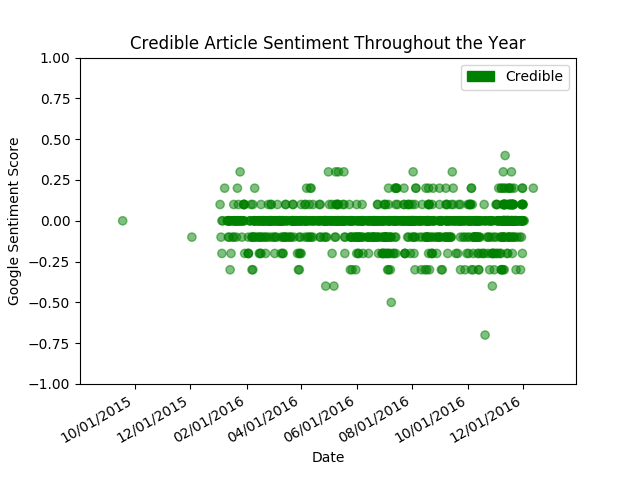
\includegraphics[width=\linewidth]{credibleSentimentThruYear.png}
            \caption{Credible Article Sentiment}
            \label{fig:credibleSentimentThruYear}
    \end{subfigure}\hfill
    \begin{subfigure}[h]{0.5\textwidth}
            \centering
            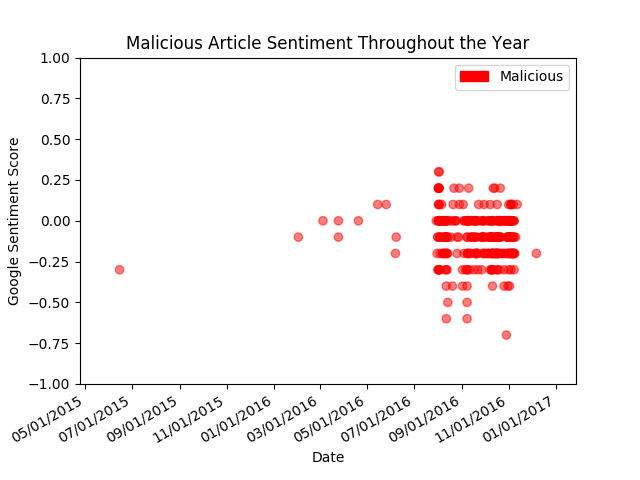
\includegraphics[width=\linewidth]{maliciousSentimentThruYear.png}
            \caption{Malicious Article Sentiment}
            \label{fig:maliciousSentimentThruYear}
    \end{subfigure}\hfill
    \caption[Article Sentiment Through Time]{
        Articles' sentiment from late 2015 to late 2016
    }
\label{fig:sentimentThruYear}
\end{figure}


Lastly, Fig. \ref{fig:sentimentThruYear} shows that distribution of Google Cloud sentiment scores throughout the date range encapsulated by the dataset.  Though most of the articles in both classes have Google sentiment scores that are relatively neutral, the proportion of malicious articles that are polar is substantially greater than the proportion of credible articles that are polar.  Only 48 of the 1008 credible articles (about 5\%) have a polar sentiment score.  On the other hand, 44 of the 333 malicious articles, or approximately 13\%, have an overall polar sentiment score.  This is a surprising statistic since credible articles also tend to have much higher sentiment magnitude.  One reason for this may be that traditional journalists try to avoid using hyperboles and stirring emotional responses \cite{opensources}.  Since the journalists who authored the credible articles tend to balance their usage of polarizing words, their articles should be more neutral than articles written by unscrupulous authors, like the Russian nationals who sought to undermine the campaigns \cite{russianBots}.

\section{Evaluation Metrics} \label{evaluationMetricsSection}

There are a variety of metrics for quantifying the performance of machine learning classifiers.  Some well-known metrics used to evaluate a classifier are overall accuracy,  precision, recall, and F1-score.  The overall accuracy (Eq. \ref{eq:overallAccuracy}), which is simply the proportion of correct classifications, is not an ideal evaluation metric for applications with large class imbalances since high accuracy scores can easily be obtained by just labelling all test documents as the class with the greatest population density.  Since the proportion of credible articles is much greater than the proportion of malicious articles, a classifier with a moderately high accuracy can still turn out to be a poor detector of malicious articles.  Thus, this study will highlight each classifier's class and prevalence-weighted average precision, recall, and F1-score due to their relationship between the number of true positives ($t_{p}$), false positives ($f_{p}$), and false negatives ($f_{n}$) produced by the classifier\cite{pythonMetrics}.

\begin{equation}
\label{eq:overallAccuracy}
\mbox{overall accuracy} = \frac{t_{p}(\mbox{credible}) + t_{p}(\mbox{malicious})}{N}, N = \mbox{size of test set}
\end{equation}
\begin{equation}
\label{eq:classPrecision}
\mbox{precision}_{c} = \frac{t_{p, c}}{t_{p, c} + f_{p, c}}
\end{equation}
\begin{equation}
\label{eq:classRecall}
\mbox{recall}_{c} = \frac{t_{p, c}}{t_{p, c} + f_{n, c}}
\end{equation}
\begin{equation}
\label{eq:classF1Score}
\mbox{F1-score}_{c} = 2 \cdot \frac{\mbox{precision}_{c} \cdot \mbox{recall}_{c}}{\mbox{precision}_{c} + \mbox{recall}_{c}}
\end{equation}
\begin{equation}
\label{eq:classProportion}
p_{c} = \frac{|D_{c}|}{N} = \frac{\mbox{number of test articles of class}\ c}{\mbox{number of test articles}}
\end{equation}
\begin{equation}
\label{eq:avgPrecision}
\mbox{weighted avg. precision} = (\mbox{precision}_{c_{0}}*p_{c_{0}}) + (\mbox{precision}_{c_{1}}*p_{c_{1}})
\end{equation}
\begin{equation}
\label{eq:avgRecall}
\mbox{weighted avg. recall} = (\mbox{recall}_{c_{0}}*p_{c_{0}}) + (\mbox{recall}_{c_{1}}*p_{c_{1}})
\end{equation}
\begin{equation}
\label{eq:avgF1Score}
\mbox{weighted  avg. F1-score} = (\mbox{F1-score}_{c_{0}}*p_{c_{0}}) + (\mbox{F1-score}_{c_{1}}*p_{c_{1}})
\end{equation}


The class precision (Eq. \ref{eq:classPrecision}) is the ratio of the true positives to the total number of predicted positives and indicates how often the classifier's prediction of a class was accurate.  The class recall (Eq. \ref{eq:classRecall}), also known as the sensitivity, is the ratio of true positives to total number documents in the class.  The recall of a class is indicative of the classifier's ability to find all the documents of that class.  To combine both the precision and recall, the class F1-score (Eq. \ref{eq:classF1Score}) is computed as the harmonic mean of both.  Finally, the prevalence-weighted average of each of these scores (Eq. \ref{eq:avgPrecision} - \ref{eq:avgF1Score}) is computed using the sum of each class score weighted by its class proportion (Eq. \ref{eq:classProportion}).  Thus, the average F1-score will be used to decide which approach works best since the average score proportionally reflects the performance of the model on each class of articles.


\section{Model Construction and Evaluation} \label{modelConstruction}

Using the training, tuning, and testing sets described in Section \ref{datasetConstruction}, we trained and evaluated the KNN, SVM, and LSTM algorithms.  The following subsections discuss how each classifier was tuned to obtain the optimal performance, and state the results of each classifier.


\subsection{$K$-Nearest Neighbor} \label{KNNResults}

The central parameter of the KNN classifier, introduced in Section \ref{knnSection}, is $k$, the number of closest neighbors used to predict the class for each document in the test set.  To train the baseline KNN classifier, only the tf-idf weights of each document were used as input.  This baseline was then trained and tested with a variety of values for $k$, as well as Euclidean distance, Manhattan distance, and cosine distance as the comparison metric, to determine the optimal model.  This tf-idf model was constructed using each article's textual content after it was preprocessed to ensure that it was converted to lowercase and tokenizable by whitespace.  Surprisingly, the optimal baseline KNN model for this setting used only 1 neighbor ($k$ = 1) and the Euclidean distance metric.  This KNN model managed to achieve an overall accuracy of 0.75 and an average F1-score of 0.71 (refer to Table \ref{table:baselineKNN} for the complete classification report using the metrics discussed in Section \ref{evaluationMetricsSection}).  For the exact number of true positives, false positives, and false negatives for each class, refer to the confusion matrix in Table \ref{table:baselineKNNConfusion}.


\begin{table}[h!]
\centering
\begin{tabular}{|c | c  c  c | c|}
\hline
class      & precision & recall & F1-score & support\\
\hline
credible   & 0.73      & 1.00   & 0.84     & 234    \\
malicious  & 0.97      & 0.30   & 0.46     & 126    \\
\hline
average    & 0.81      & 0.75   & 0.71     &   \\
\hline
\end{tabular}
\caption[Baseline KNN's Classification Report]{Classification results of the baseline KNN model (trained using only the tf-idf weights as the input feature vector, $k$ = 1, and the Euclidean distance metric)}
\label{table:baselineKNN}
\end{table}


\begin{table}[h!]
\centering
\begin{tabular}{|c | c  c | c|}
\hline
                Actual class & 
                Predicted credible 
                &   
                Predicted malicious
                & support\\
\hline
credible   & 233                & 1                   & 234\\
malicious  & 88                 & 38                  & 126\\
\hline
total      & 321                & 39                  & 360\\
\hline
\end{tabular}
\caption[Baseline KNN's Confusion Matrix]{Confusion matrix for the baseline KNN model}
\label{table:baselineKNNConfusion}
\end{table}


The next KNN classifier was trained using feature vectors composed of the number of characters, number of words, Google sentiment score, Google sentiment magnitude, and Microsoft sentiment score of each training article.  The optimal model, which used $k$ = 5 and Manhattan distance, obtained an overall accuracy of 0.75 and an average F1-score of 0.72 (refer to Table \ref{table:secondKNN} for class-specific metrics).


\begin{table}[h]
\centering
\begin{tabular}{|c | c  c  c | c|}
\hline
class      & precision & recall & F1-score & support\\
\hline
credible   & 0.74      & 0.93   & 0.83     & 234    \\
malicious  & 0.76      & 0.40   & 0.53     & 126    \\
\hline
average    & 0.75      & 0.75   & 0.72     &   \\
\hline
\end{tabular}
\caption[Second KNN's Classification Report]{Classification results of the second KNN model (trained using all of the sentiment features, as well as the word and character counts, $k$ = 5, and the Manhattan distance metric)}
\label{table:secondKNN}
\end{table}


\begin{table}[h!]
\centering
\begin{tabular}{|c | c  c  c | c|}
\hline
class      & precision & recall & F1-score & support\\
\hline
credible   & 0.75      & 0.94   & 0.83     & 234    \\
malicious  & 0.79      & 0.42   & 0.55     & 126    \\
\hline
average    & 0.76      & 0.76   & 0.73     &   \\
\hline
\end{tabular}
\caption[Final KNN's Classification Report]{Classification results of the final KNN model (trained using tf-idf weights of each document, the number of characters and words in the document, the Google sentiment score and magnitude for the document, and the Microsoft sentiment score, $k$ = 7, and the Euclidean distance metric)}
\label{table:lastKNN}
\end{table}


Finally, another KNN classifier was trained using the tf-idf weights vector of each document, as well as all of the sentiment and count-related features used by the second KNN.  This classifier managed to achieve an overall accuracy of 0.76 and an average F1-score of 0.73 using $k$ = 7 and Euclidean distance (refer to Table \ref{table:lastKNN} for more metric scores).


\subsection{Support Vector Machine} \label{SVMResults}

Three SVMs were trained using the same setup that was used to train the three KNNs in Section \ref{KNNResults}.  The baseline SVM used only the tf-idf weights vector of each document as the input during training and testing, the next SVM used character and word counts along with the sentiment features of each document, and the final SVM used all of the features including the tf-idf weights.


\begin{table}[h]
\centering
\begin{tabular}{|c | c  c  c | c|}
\hline
class      & precision & recall & F1-score & support\\
\hline
credible   & 0.85      & 1.00   & 0.92     & 234    \\
malicious  & 1.00      & 0.67   & 0.81     & 126    \\
\hline
average    & 0.90      & 0.89   & 0.88     &   \\
\hline
\end{tabular}
\caption[Baseline SVM's Classification Report]{Classification results of the baseline SVM model (trained using only the tf-idf weights of each document, a linear kernel function, and $C$ = 1.0)}
\label{table:baselineSVM}
\end{table}


\begin{table}[h]
\centering
\begin{tabular}{|c | c  c | c|}
\hline
                Actual class & 
                Predicted credible 
                &   
                Predicted malicious
                & support\\
\hline
credible   & 234                & 0                   & 234\\
malicious  & 41                 & 85                  & 126\\
\hline
total      & 275                & 85                  & 360\\
\hline
\end{tabular}
\caption[Baseline SVM's Confusion Matrix]{Confusion matrix for the baseline SVM model}
\label{table:baselineSVMConfusion}
\end{table}


The optimal baseline SVM achieved an overall accuracy of 0.89 and an average F1-score of 0.88 using a linear kernel function, and regularization parameter ($C$) of 1.0 \cite{svcDoc}.  For a complete summary of the performance of the baseline SVM, refer to Table \ref{table:baselineSVM}.  Note that the performance of this baseline is much better than that of the baseline KNN (recall that the baseline KNN achieved an average F1-score of just 0.71).  The confusion matrix in Table \ref{table:baselineSVMConfusion} provides an explanation for this phenomenon: every credible article was correctly identified by the SVM, and more than twice as many malicious articles were successfully detected by the SVM than the KNN.

Unlike the improvement that the second KNN showed over the baseline KNN, the second SVM, trained without the tf-idf weights, performed significantly worse than the baseline SVM.  The overall accuracy of this new SVM model was 0.75, and its average F1-score was only 0.71.  This model used a radial basis kernel function, gamma of 0.0005 (the coefficient on the radial basis kernel), and $C$ = 1.0 (refer to Table \ref{table:secondSVM} for a complete summary of the SVM's performance).


\begin{table}[h!]
\centering
\begin{tabular}{|c | c  c  c | c|}
\hline
class      & precision & recall & F1-score & support\\
\hline
credible   & 0.73      & 0.96   & 0.83     & 234    \\
malicious  & 0.82      & 0.36   & 0.50     & 126    \\
\hline
average    & 0.76      & 0.75   & 0.71     &   \\
\hline
\end{tabular}
\caption[Second SVM's Classification Report]{Classification results of the second SVM model (trained using all of the sentiment features, as well as the word and character counts, a radial basis function, gamma = 0.0005, and $C$ = 1.0)}
\label{table:secondSVM}
\end{table}


The final SVM, which used each document's tf-idf weights in conjunction with the number of characters and words, and the Google and Microsoft sentiment features for the document, showed slight improvement over the second SVM.  This SVM, trained with a radial basis function, a gamma of 0.0001, and $C$ = 0.5, ultimately obtained an overall accuracy of 0.76 and an average F1-score of 0.73.  For the class precision, recall, and F1-scores, refer to Table \ref{table:lastSVM}.


\begin{table}[h]
\centering
\begin{tabular}{|c | c  c  c | c|}
\hline
class      & precision & recall & F1-score & support\\
\hline
credible   & 0.75      & 0.97   & 0.84     & 234    \\
malicious  & 0.86      & 0.39   & 0.54     & 126    \\
\hline
average    & 0.79      & 0.76   & 0.73     &   \\
\hline
\end{tabular}
\caption[Final SVM's Classification Report]{Classification results of the final SVM model (trained using tf-idf weights of each document, the number of characters and words in the document, the Google sentiment score and magnitude for the document, and the Microsoft sentiment score, a radial basis function, gamma = 0.0005, and $C$ = 1.0)}
\label{table:lastSVM}
\end{table}


\subsection{Long Short-Term Memory Network}

The last model evaluated in this study was the LSTM.  As discussed in Section \ref{rnnSection}, LSTMs have proven to be successful in tasks involving sequential information because of their memory units.  However, the input vectors used with the other classifiers, such as the tf-idf weights vector, do not retain any information about the sequential relationship between the words and sentences that make up each document.  Thus, the more reasonable input for LSTMs are sequences of word embedding vectors; in fact, word embeddings are the preferred choice for textual representation in modern deep learning \cite{wordEmbedding}.

Using the training and tuning set, we tuned LSTM's number of memory units, number of epochs, batch size, and input and recurrent dropout rates.   The number of epochs is the number of times the entire training set is passed forward and backward through the neural network.  If the number of epochs is too low, the network may be underfit and the resulting neuron weights will be far from optimal.  The batch size is simply the number of samples fed into the network before each update to the weights and helps to make training more efficient by reducing the memory requirements and the number of iterations required to reach the optimal weights \cite{batchSize}.  Finally, the dropout rate is simply probability that an input or recurrent node is excluded from consideration during a weight update in an effort to reduce overfitting \cite{dropoutRate}.


\begin{table}[h]
\centering
\begin{tabular}{|c | c  c  c | c|}
\hline
class      & precision & recall & F1-score & support\\
\hline
credible   & 0.90      & 0.95   & 0.93     & 234    \\
malicious  & 0.90      & 0.80   & 0.85     & 126    \\
\hline
average    & 0.90      & 0.90   & 0.90     &   \\
\hline
\end{tabular}
\caption[LSTM's Classification Report]{Classification results of the top-performing LSTM (overall accuracy of 0.90) using batch size of 24, 8 epochs, dropout rate of 0.5, and 50 memory units}
\label{table:lstmResults}
\end{table}

\begin{table}[h]
\centering
\begin{tabular}{|c | c  c | c|}
\hline
                Actual class & 
                Predicted credible 
                &   
                Predicted malicious
                & support\\
\hline
credible   & 223                & 11        & 234\\
malicious  & 25                 & 101       & 126\\
\hline
total      & 256                & 104       & 360\\
\hline
\end{tabular}
\caption[LSTM Confusion Matrix]{Confusion matrix for the LSTM model trained using 50 memory units, batch size of 24, a dropout rate of 0.5, and 8 epochs}
\label{table:lstmConfusion}
\end{table}

As illustrated by Table \ref{table:lstmResults}, the LSTM achieves an overall accuracy of 0.90, as well as an average F1-score of 0.90, with just 50 memory units, a batch size of 24, and 8 epochs.  According to the LSTM's confusion matrix (Table \ref{table:lstmConfusion}), the LSTM has 11 more false negatives for the credible class of articles than the SVM model, but 16 fewer false negatives for the malicious class of articles.
